\sectionSlide{C with Classes}{young-bjarne}{1.2\paperheight}


\slide{Roots of C++}{
    \centering 
    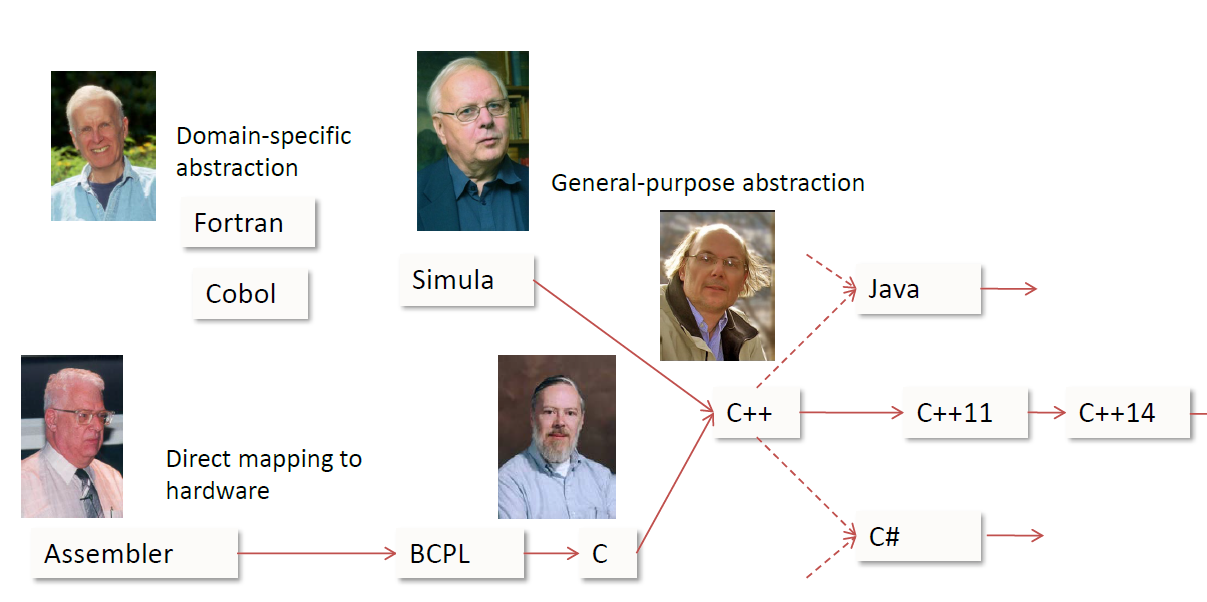
\includegraphics[height=0.8\paperheight]{cpp_roots}
    %NOTE: Before C Programming Language - Basic Combined Programming Language
}


\slide{Roots of C++}{
    Languages that were considered as a base of C++:
    \begin{itemize}
        \item Modula2
        \item Ada
        \item Smalltalk
        \item Mesa
        \item Clu
        \item C
    \end{itemize}
}


\timeSlide{C with Classes}{
    Additions to C language:
    \begin{itemize}%[<+->]
        \item classes
        \item derived classes
        \item public and private access control
        \item constructors and destructors
        \item \textbf<2>{call and return functions (removed later)}
        \item friend classes
        \item type checking and conversion of function arguments
    \end{itemize}
}{          
    \draw[thin,blue]
    (0.5, 0) node(l1979)[anchor=west,fill=green!20,rounded corners] {\textbf{1979} C with Classes};
    
    \draw[] (1979) -- (l1979);
}

\slide{Example code in C with Classes}{
    \lstinputlisting{"src/c-with-classes.hpp"}
}


\slide{Roots of C++}{
    In C++ you can see the influence of 4 languages:
    \begin{itemize}
        \item C provided all base and syntax
        \item Simula provided classes and inheritance
        \item Algol68 provided:
            \begin{itemize}
                \item operator overloading, 
                \item references 
                \item ability to declare variables anywhere in a block  %NOTE: in C you had to declare variables first
            \end{itemize}
        \item BCPL provided // comments (later in 1985).
    \end{itemize}
}


\timeSlide{First standard library}{
    \begin{itemize}
        \item complex numbers
        \item string
        \item later: iostreams
    \end{itemize}
}{          
    \draw[thin,blue]
        (0.5, 0) node(l1979)[anchor=west] {1979 C with Classes}
        (0.5,-0.4) node(l1981)[anchor=west] {1981 New features}
        (0.5,-0.8) node(l1983)[anchor=west,fill=green!20,rounded corners] {\textbf{1983} 1st std lib};
            
    \draw[]
    (1979) -- (l1979)
    (1981) -- (l1981)
    (1983) -- (l1983);
}


\slide{C with Classes - summary}{
    \begin{itemize}
        \item Years of development: 1979-1983
        \item The idea was great
        \item The aim was clear:
            \begin{itemize}
                \item help programmers to organize code with classes
                \item without the loss of efficiency 
                \item and without requiring from users learning something completely new
            \end{itemize}
        \item C with Classes didn't have many users :( 
        \item It wouldn't pay to support this language in the form it was
        \item C with Classes was a "medium success"
    \end{itemize}
    Bjarne knew about it and drawn conclusions.
}
